\documentclass[11pt]{article}
\usepackage{preamble}
\usepackage[]{gset}
\def\week{12}
\def\theproblem{К\week.\arabic{problem}}

\begin{document}
	
	\newpage
	\setcounter{problem}{0}
	\def\theproblem{Д\week.\arabic{problem}}
	{\textbf{\large Дискретная математика}\hfill \textbf{(Основной поток)}
		
		\medskip %
		
		\textbf{Домашнее задание \week}}
	
	\medskip
	
	\textbf{Дайте обоснованные ответы на следующие вопросы.}
	
	
	\vspace{5mm}
	
	
	
	\p Докажите, что можно так занумеровать вершины связного
	неориентированного графа на $n$ вершинах числами от 1 до $n$, что для
	каждого $1\leq k\leq n$ связен подграф, индуцированный множеством вершин с
	номерами от 1 до $k$. 
	
	Множество $S$ вершин графа $G = (V,E)$ индуцирует  подграф с
	множеством вершин $S$,  рёбрами которого являются все рёбра из $E$ с обоими концами в~$S$.
	
	Зададим обход в глубину по вершинам графа со стартом в произвольной вершине $v$. Будем присваивать каждой новой вершине новый наименьший доступный номер. Так как изначальный граф связен, получим остовное дерево с корнем в вершине $v$. Для каждой вершины будет существовать путь до корня, номера вершин на пути будут убывать. Пусть дано $k$, тогда любой путь из вершин с номерами $q \leq k$ входит в индуцированный подграф, потому что номера вершин на нем уменьшаются. Получаем, что в подграфе каждая вершина связана с $v$, значит подграф связен. 
	
	\p Найдите такой граф на 8 вершинах, что степень каждой вершина равна~3 и
	в этом графе нет независимого множества размера~4. (Напомним, что, как
	и во всех остальных задачах, ответ должен быть обоснован. Нужно
	доказать, что ваш пример удовлетворяет требуемым свойствам.)
	
	\[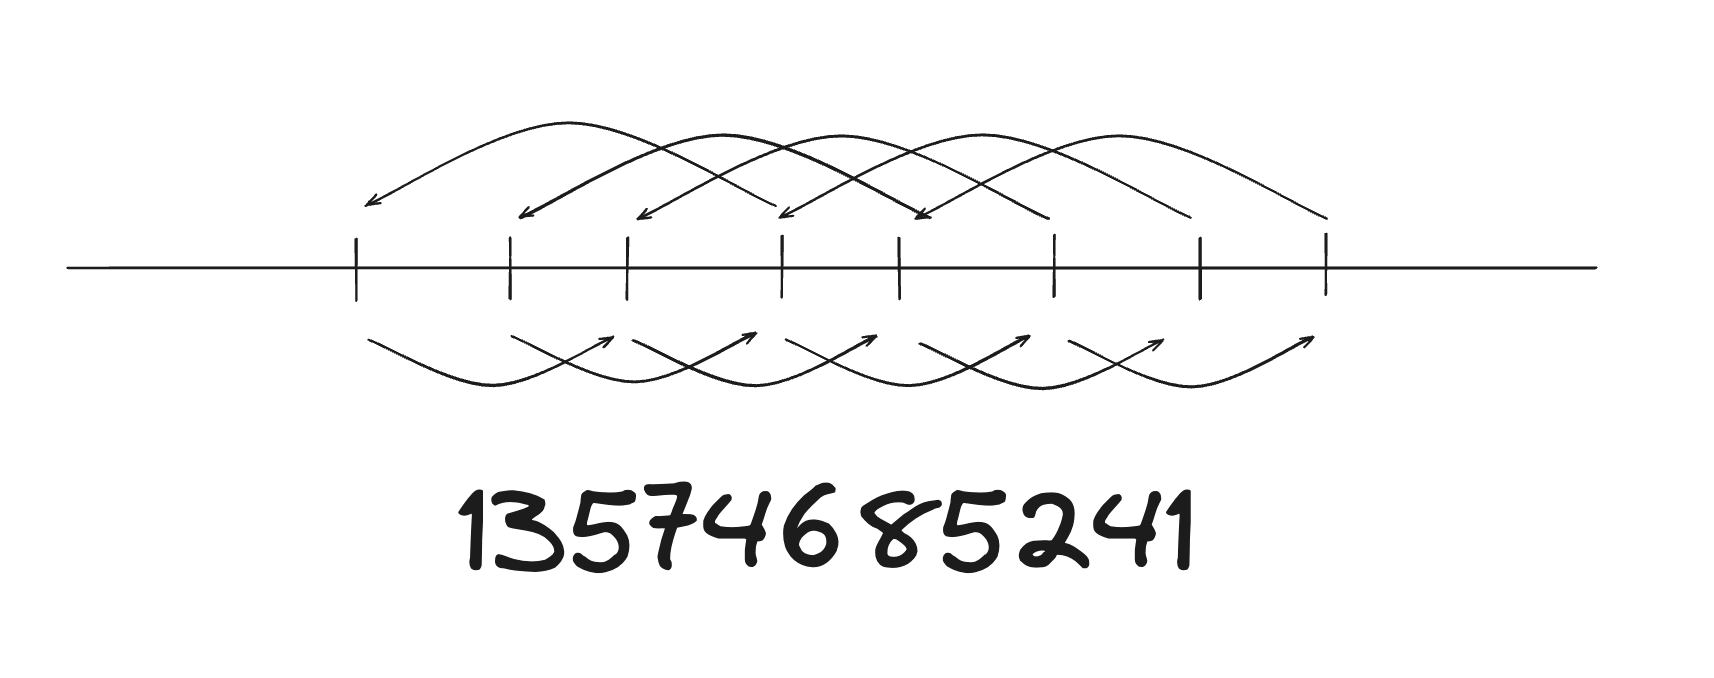
\includegraphics[width=75mm]{img}\]
	
	Из каждой компоненты связности можно взять только по одной вершине, получается, что размер независимого множества не больше 2. 
	
	\p Известно, что в простом неориентированном графе нечётное количество независимых множеств. Следует ли из этого, что граф связный?
	(Независимое множество~"--- это подмножество вершин, в котором каждая пара вершин не соединена ребром. Пустое множество и 1"=элементные множества являются  независимыми.)
	
	Контрпример 
	\[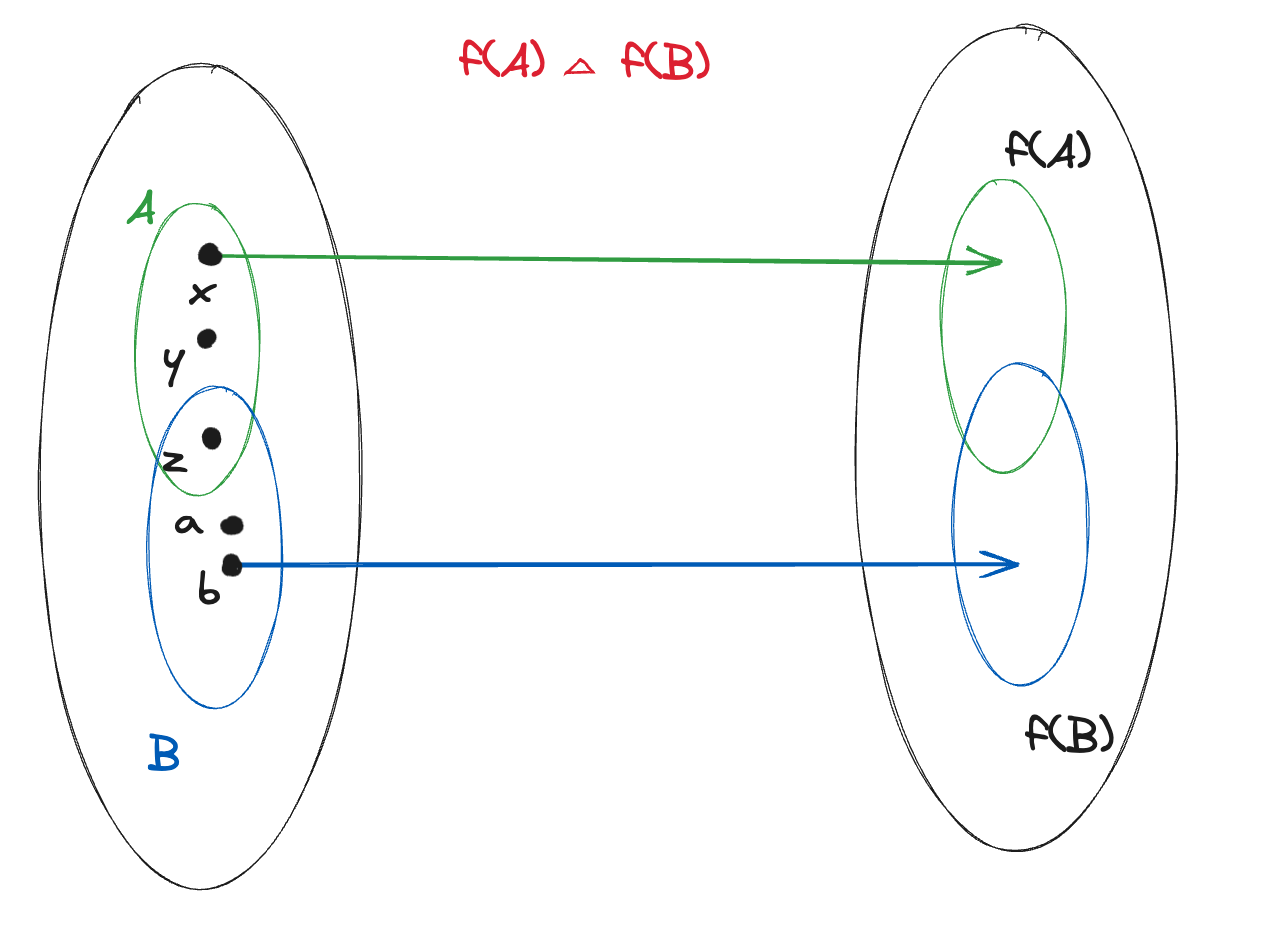
\includegraphics[width=40mm]{img3}\]
	
	Независимых множеств 9, но граф не связный.
	
	\p При каких $n$ в булевом кубе $Q_n$ существует остовное дерево, в котором все вершины кроме двух имеют степень~2?
	
	При всех $n \in \mathbb{N}$. Приведем алгоритм построения остовного дерева. Для $n = 2$ построим дерево: \\ 0 - 1. При увеличении n допишем для уже имеющегося пути 0 в конец каждого члена, получим $00 - 10$. Мы не нарушим путь, потому что дописываем одинаковые символы. Теперь соединим последний член пути с ним же, только где последний разряд 1. Ребро есть, потому что они отличаются только последним разрядом. Теперь пройдемся по предыдущему пути для $n - 1$ в обратном порядке, к каждому члену пути будем дописывать 1 в конец: $00 - 10 - 11 - 01$. Путь есть, потому что дописываем одно и то же \\
	Для $n = 3: 000 - 100 - 110 - 010 - 011 - 111 - 101 - 001$.  \\
	Для $n = 4: 0000 - 1000 - 1100 - 0100 - 0110 - 1110 - 1010 - 0010 - 0011 - 1011 - 1111 - 0111 - 0101 - 1101 - 1001 - 0001$
	
	\[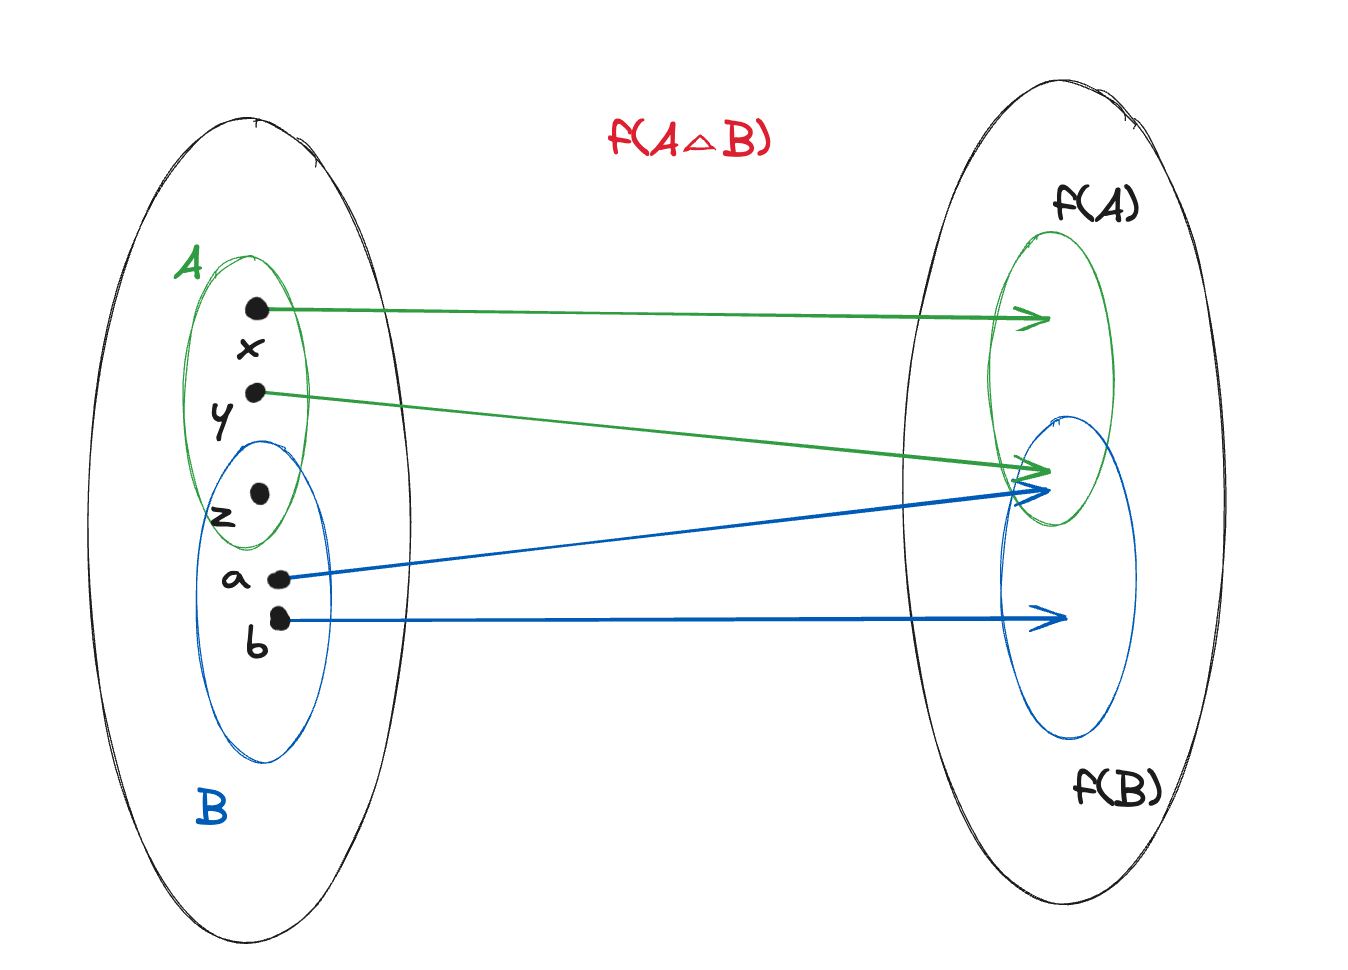
\includegraphics[width=75mm]{img2}\]
	
\end{document}